\subsection{Abstract Factory Pattern}
The abstract factory pattern is present in the \texttt{Factory} class. In the repository, the class can be located at \texttt{factory.h}. The class is used to create several concrete products, including \texttt{Component} and \texttt{Module} objects.

Figure \ref{fig:af} lists the methods of the class following the typical steps dictated by the pattern.

\begin{figure}[h]
    \caption{Factory Implementing the Abstract Factory Pattern}
    \label{fig:af}
    \centering
    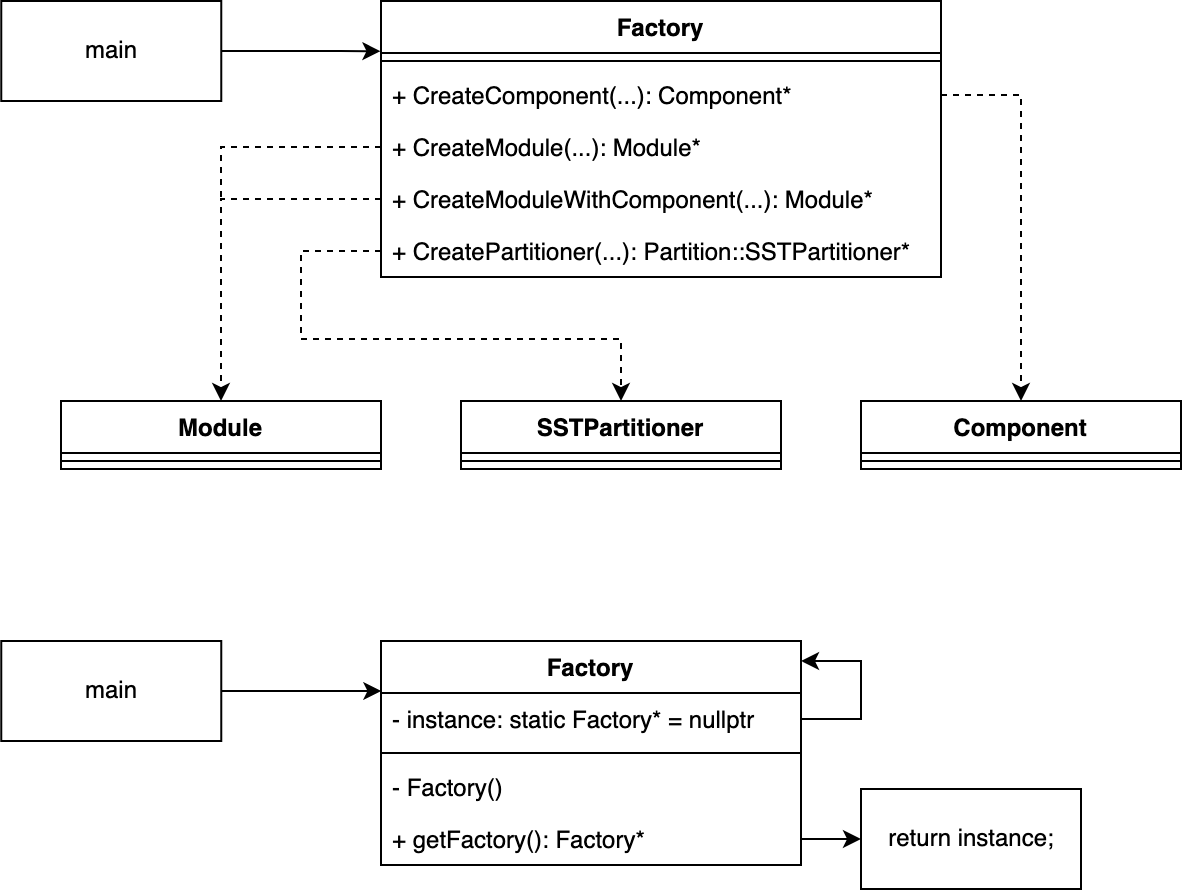
\includegraphics[width=0.8\textwidth]{af.png}
\end{figure}

Each of the methods accept parameters to instantiate the corresponding ConcreteProducts. There are several Client classes that call these methods, including \texttt{Simulation}, \texttt{BaseComponent} and the \texttt{main} function itself.
